\documentclass{article}
\usepackage{ctex}
\usepackage{graphicx}
\usepackage{ctex}
\usepackage{amsmath}
\usepackage{amsfonts}
\usepackage{amssymb}
\usepackage{enumerate}
\usepackage{color}
\usepackage{setspace}
\usepackage{pythonhighlight}
\usepackage{bm}

\usepackage
[a4paper,
text={146.4true mm,239.2 true mm},
top= 26.2true mm,
left=31.8 true mm,
head=6true mm,
headsep=6.5true mm,
foot=16.5true mm]
{geometry} % 设置文本的边距
\input{../setup/format}

\begin{document}
    \title{Homework 3 of Stochastic Processes}
    \author{姓名:林奇峰\qquad 学号:19110977}
    \maketitle

    请参考教材 Figure 2.1,编写程序仿真。分别画5个$n=10$的样本函数,体会到达过程和泊松过程。
    \begin{enumerate}[1)]
        \item 更新过程,间隔时间通过掷一枚均匀骰子决定,掷到多少点间隔就取多少。
        \item 更新过程,间隔时间服从$[0,1]$上的均匀分布。
        \item 泊松过程$\lambda=1$。  
    \end{enumerate}

    \noindent\textbf{Solutions:}

    \begin{enumerate}[1)]
        \item 通过掷骰子来决定时间间隔的更新过程样本函数图像如图\ref{fig:dices}所示:
            \begin{figure}[h]
                \centering
                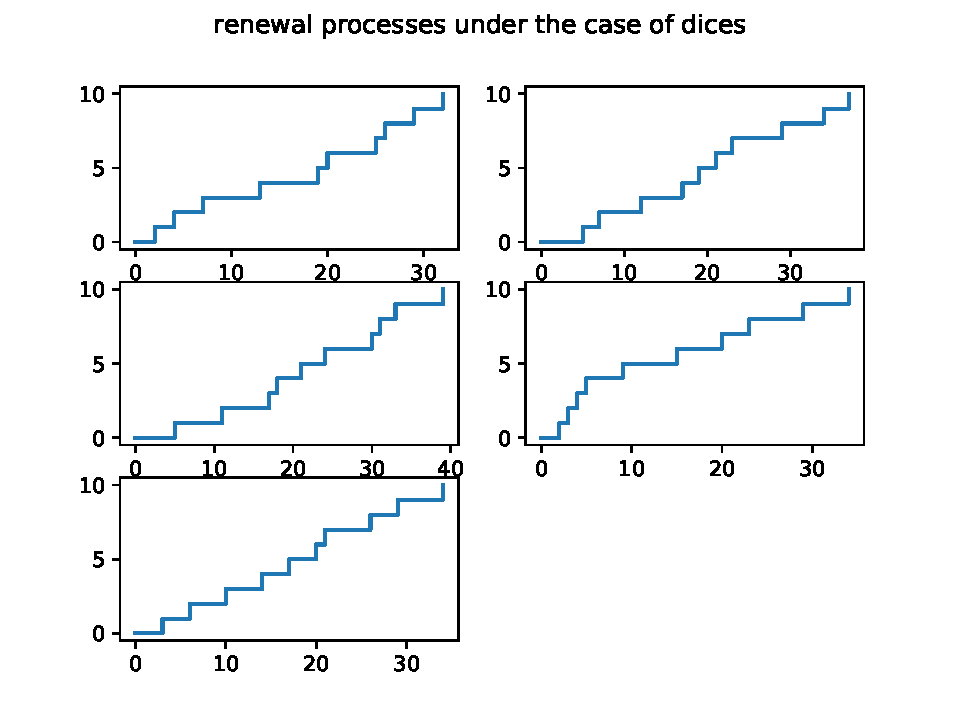
\includegraphics[width=6.0in]{dices.pdf}
                \caption{通过掷骰子来决定时间间隔的更新过程样本函数}
                \label{fig:dices}
            \end{figure}
    \end{enumerate}

    \clearpage
    \begin{enumerate}[2)]
        \item 通过$[0,1]$均匀分布来决定时间间隔的更新过程样本函数图像如图\ref{fig:uniform}所示:

            \begin{figure}[h]
                \centering
                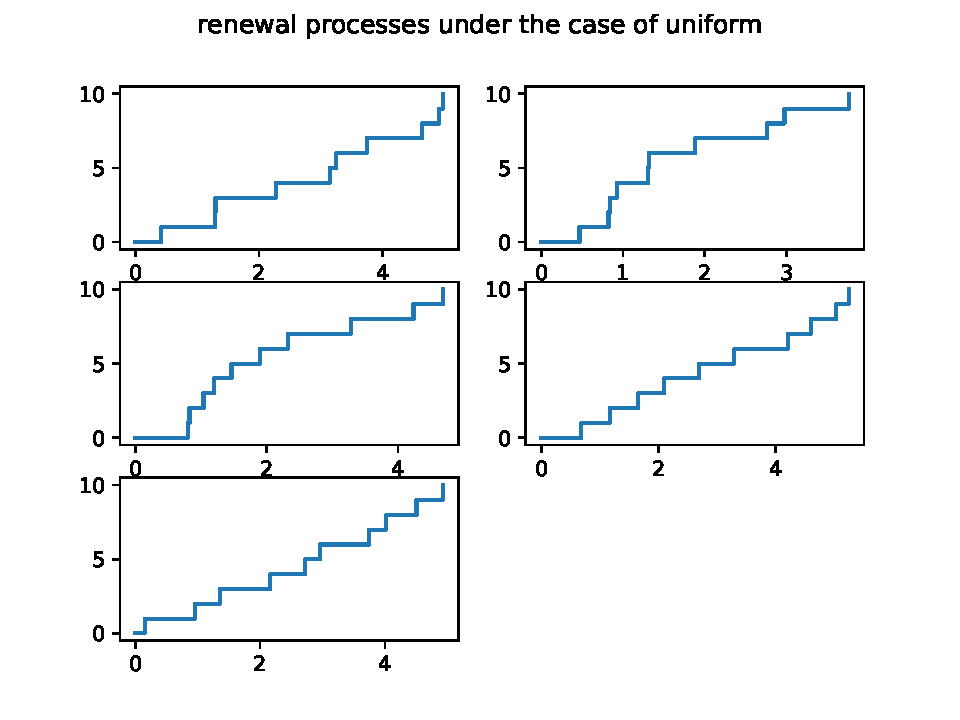
\includegraphics[width=6.0in]{uniform.pdf}
                \caption{通过$[0,1]$均匀分布来决定时间间隔的更新过程样本函数}
                \label{fig:uniform}
            \end{figure}
    \end{enumerate}
    \clearpage
    \begin{enumerate}[3)]
        \item 泊松过程的样本函数图像如图\ref{fig:poisson}所示:
            \begin{figure}[h]
                \centering
                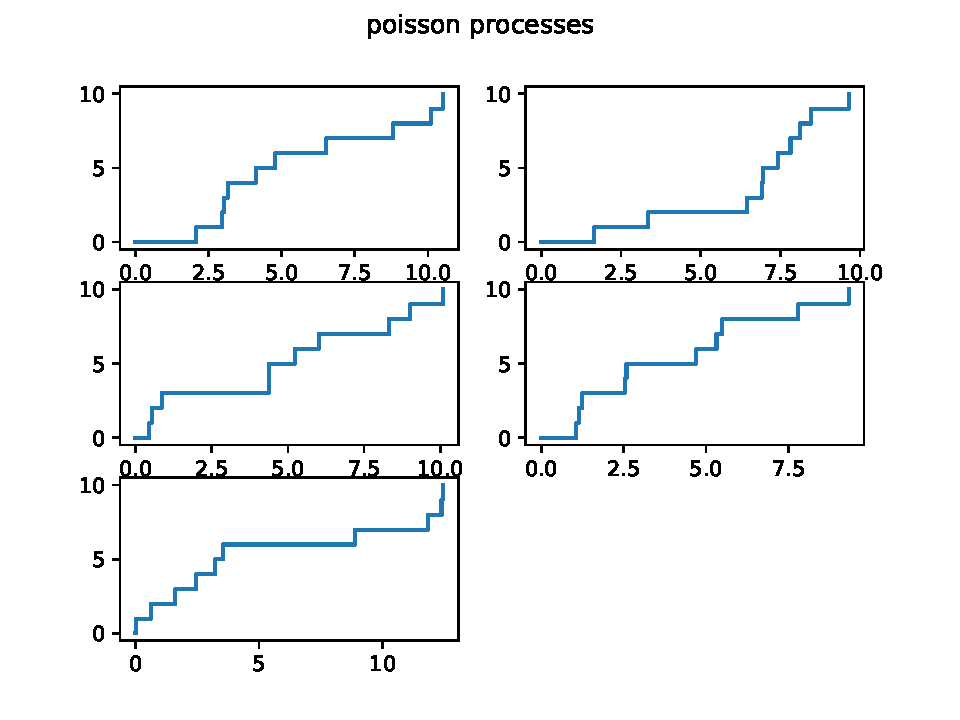
\includegraphics[width=6.0in]{poisson.pdf}
                \caption{泊松过程}
                \label{fig:poisson}
            \end{figure}
    \end{enumerate}

具体的代码如下
    \begin{python}
import numpy as np
import matplotlib.pyplot as plt
plt.rcParams['font.sans-serif'] = ['SimHei']
plt.rcParams['axes.unicode_minus'] = False 


def plot_dice(n, epoch, figure):
    plt.figure(figure)
    for i in range(epoch):
        S=[0]
        N=[0]
        X=[]
        for j in range(n):
            val = np.random.randint(low=1, high=7)
            S.append(np.sum(X) + val)
            N.append(N[-1] + 1)
            X.append(val)
        plt.subplot(3, 2, i + 1)
        plt.step(S, N, where='post')
    plt.suptitle('renewal processes under the case of dices')
    plt.show()

def plot_uniform(n, epoch, figure):
    plt.figure(figure)
    for i in range(epoch):
        S=[0.0]
        N=[0] 
        X=[]
        for j in range(n):
            val = np.random.uniform(low=0, high=1.0)
            S.append(np.sum(X) + val)
            N.append(N[-1] + 1)
            X.append(val)
        plt.subplot(3, 2, i + 1)
        plt.step(S, N, where='post')
    
    plt.suptitle('renewal processes under the case of uniform')
    plt.show()

def plot_possion(n, epoch, figure):
    plt.figure(figure)
    for i in range(epoch):
        S=[0.0]
        N=[0]
        X=[]
        for j in range(n):
            val = np.random.exponential(scale=1.0)
            S.append(np.sum(X) + val)
            N.append(N[-1] + 1)
            X.append(val)
        plt.subplot(3, 2, i + 1)
        plt.step(S, N, where='post')
    plt.suptitle('poisson processes')
    plt.show()


if __name__ == "__main__":
    epoch = 5
    n = 10

    plot_dice(n, epoch, figure=1)
    plot_uniform(n, epoch, figure=2)
    plot_possion(n, epoch, figure=3)
    
    \end{python}
\end{document}